\section{Assignment 5}

\subsection{Compute the 3D trajectory (position, velocity, acceleration and jerk) in the picture as
a combination of linear and circular motion primitives and compare it with the
trajectory obtained using one of the multi-point methods.}

\begin{figure}[h]
\centering
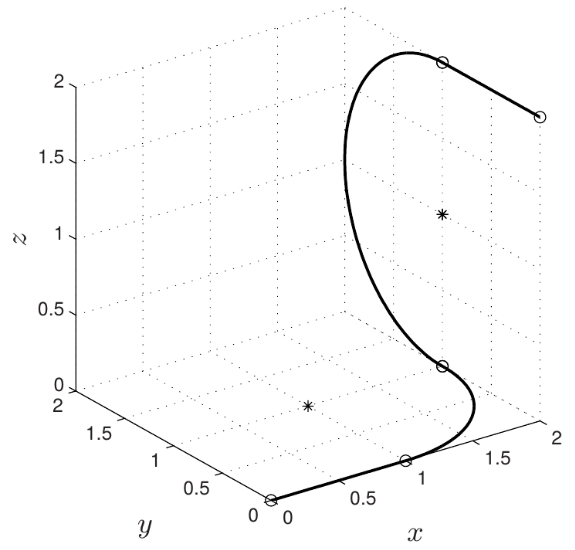
\includegraphics[keepaspectratio,width=0.35\textwidth]{3Dtraj_ref}
\caption{3D trajectory - reference.}
\end{figure}

Operational space trajectories can be computed by composing multiple motion primitives. The motion primitives used here are:

\begin{itemize}
\item Rectilinear path:
\begin{equation*}
p(u)=p_i+u(p_f-p_i)\;\;\;\;\;u\in[0,1]
\end{equation*}
\item Circular path:
\begin{equation*}
p(u)=c+Rp'(u)=c+R\begin{bmatrix}
\rho\cos(u)\\\rho\sin(u)\\
0
\end{bmatrix}=c+\begin{bmatrix}
(P-c)' & e_3'\cross(P-c)' & e_3'
\end{bmatrix}\begin{bmatrix}
\rho\cos(u)\\\rho\sin(u)\\
0
\end{bmatrix}\;\;\;\;\;u\in[0,\theta]
\end{equation*}

where $c$ is the position of the center of the circular path, $P$ is the position of the starting point on the circle and $e_3=\begin{bmatrix}
0 & 0 & 1
\end{bmatrix}$.
\end{itemize}

For comparison, a 3D trajectory is computed by computing the smoothing cubic splines along the three directions. The smoothing spline trajectory is also computed with added waypoints to improve the tracking of the position.

\begin{figure}[H]
\centering
\includegraphics[keepaspectratio,width=0.4\textwidth]{3Dtraj}
\caption{3D trajectory - motion primitives vs smoothing splines ($w_k=\infty\forall k$, $\mu=1$).}
\end{figure}

\begin{figure}[h]
\centering
\includegraphics[keepaspectratio,width=0.6\textwidth]{3Dtraj_pos}
\caption{3D trajectory - Position comparison.}
\end{figure}

\begin{figure}[h]
\centering
\includegraphics[keepaspectratio,width=0.9\textwidth]{3Dtraj_profiles}
\caption{3D trajectory - Velocity, acceleration, jerk comparison.}
\end{figure}